\documentclass[11pt]{beamer}
\usepackage{tcolorbox}
\usepackage{multicol}
\usepackage[export]{adjustbox}
\usepackage{tikz}
\usepackage{minted}
\usepackage{amssymb}
\usemintedstyle{gruvbox-light}
\newcommand{\R}[1]{\mintinline[escapeinside=||]{r}{#1}}
\usepackage{mathrsfs}

\usepackage{array,booktabs,ragged2e}
\setlength{\RaggedRightRightskip}{0pt plus 9em}
\newcolumntype{R}[1]{>{\RaggedRight\arraybackslash}p{#1}}

\newcommand*{\tc}[2]{%
    \textcolor{#1}{#2}
}

\newcommand*{\gr}[1]{%
    {\small \textcolor{gray}{#1}}
}


\newcommand*{\colitem}[2]{%
    \item[\textcolor{#1}{\textbullet}] \textcolor{#1}{#2}
}

\newcommand{\sgap}{\vspace{0.5em}}
\newcommand{\bgap}{\vspace{0.8em}}

\newcommand\Wider[2][3em]{%
\makebox[\linewidth][c]{%
  \begin{minipage}{\dimexpr\textwidth+#1\relax}
  \raggedright#2
  \end{minipage}%
  }%
}

% Fonts --------------------------------------------------------------------------

\usepackage[scaled]{helvet}
\usepackage[T1]{fontenc}
\usepackage[utf8]{inputenc}
\usepackage[scale=0.95]{inconsolata}

% References ------------------------------------------------------------------

\usepackage[%
  backend     = biber,
  style       = numeric,
  sorting     = ynt,
  sortcites   = true,
  autocite    = superscript
]{biblatex}

\addbibresource{references.bib}

% tcolorbox -------------------------------------------------------------------

\newtcolorbox{cbox}[3][]
{
  colframe = #2!5,
  colback  = #2!5,
  coltitle = #2!50!black,  
  colbacktitle = #2!5,
  lefttitle = 1mm,
  toptitle = 2mm,
  bottomtitle = 0mm,
  colupper = #2!50!black,  
  title    = {#3},
  fonttitle = \bfseries\large,
  #1,
  arc=0.5mm,
  left=2.5mm,
  before upper={\setbeamercolor{item}{fg=#2!50!black}},
  after upper={\setbeamercolor{item}{fg=#2!50!black}}
}

\makeatletter
\def\beamer@origitem{%
  \@inmatherr\item\@ifnextchar[\@item{\@noitemargtrue\@item[\@itemlabel]%
  \csname beamer@thcfg@\beameritemnestingprefix item\endcsname% Insert colour in \beamer@thc@fg
  \ifx\beamer@thc@fg\@empty\relax\else\color{\beamer@thc@fg}\fi% Execute colour
  }}
\makeatother

\usepackage{graphicx}
\newcommand*{\img}[1]{%
    \raisebox{-.3\baselineskip}{%
        \includegraphics[
        height=\baselineskip,
        width=\baselineskip,
        keepaspectratio,
        ]{#1}%
    }%
}

\newcommand*{\timg}[2]{%
	\raisebox{-.5#1}{%
		\includegraphics[
			width=#1
		]{#2}%
    }%
}

\title[The pmsims package for R]{
    A simulation approach to calculating minimum sample sizes for prediction
    modelling
}
\subtitle{The pmsims package for R}
\date{29$^{\text{th}}$ August 2023}
\author[Biostatistics \& Health Informatics, KCL]{%
    Ewan Carr, Gordon Forbes, Diana Shamsutdinova, \mbox{Daniel Stahl},
	and Felix Zimmer}
\institute[]{Department of Biostatistics \& Health Informatics\\ King's College London}
\titlegraphic{
\includegraphics[height=1.5cm]{figures/kcl.png}}
\setbeamertemplate{navigation symbols}{}
\setbeamertemplate{footline}[frame number]

% Theme
\definecolor{KCLpurple}{RGB}{80, 20, 145}
\definecolor{KCLred}{RGB}{226, 35, 26}
\definecolor{KCLhotpink}{RGB}{200, 50, 150}
\definecolor{KCLpurple}{RGB}{80, 20, 145}
\definecolor{KCLseablue}{RGB}{0, 90, 210}
\definecolor{KCLtealblue}{RGB}{0, 154, 166}
\definecolor{KCLpeagreen}{RGB}{0, 181, 136}
\definecolor{KCLpantone}{RGB}{0, 35, 149}
\usecolortheme[named=KCLseablue]{structure}
\setbeamercolor{alerted text}{fg=KCLhotpink}

\setbeamertemplate{itemize items}[circle]
\setbeamertemplate{enumerate items}[default]

\newenvironment{itemize*}%
{\begin{itemize}%
		\setlength{\itemsep}{100pt}%
		\setlength{\parskip}{0pt}}%
		{\end{itemize}}

\begin{document}

\maketitle

\begin{frame}[c]
	\vspace{1em}
	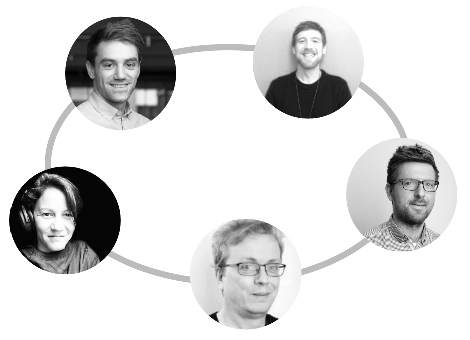
\includegraphics[width=\textwidth]{figures/group_photos.pdf}%
\end{frame}


\section{Introduction}

\begin{frame}[c]{30-second version}
	\Large
	\begin{enumerate}
		\setlength{\itemsep}{12pt}

		\item Most prediction models use small samples.

		\item Small samples cause overfitting and imprecise estimates.

		\item Existing tools can estimate minimum samples for continuous,
		      binary, and survival outcomes.

		\item Nothing exists for other models or data types.

	\end{enumerate}

	\sgap

	\begin{cbox}{KCLtealblue}{}
		We're developing a simulation-based approach that works with any
		outcome or method.
	\end{cbox}
	\vspace{-1em}
\end{frame}

\begin{frame}[t]{This talk}
    \sgap
	\Large
	\begin{enumerate}
		\item Background
		      \begin{itemize}
			      \item What's the problem we're trying to solve?
			      \item What solutions currently exist?
		      \end{itemize}
		\item Our simulation-based approach
		      \begin{itemize}
			      \item Workflow and user interface
			      \item How it compares to other packages
		      \end{itemize}
		\item Demonstration
		\item Development status and next steps
	\end{enumerate}

    \normalsize
	\vspace{6mm}
	\begin{cbox}{KCLtealblue}{}
		\centering
		
\includegraphics[width=4em,valign=c]{figures/construction-site.pdf}
		\hspace{2em} {\large Under construction; feedback welcome.}
	\end{cbox}

\end{frame}

\section{Background}

\begin{frame}[t]{Most models are developed with inadequate samples}
	% Say: Prediction models can inform treatment decisions, facilitate
	% screening, and enable stratified care.

	% risk stratification, informing, shared decision making

	% Hundreds of prediction models are developed each year. Most have
	% inadequate samples.

	\begin{cbox}[bottom=0.5mm]{KCLseablue}{}
		\begin{itemize}
			\item Small samples the most common cause of bias in 731 models
			      for COVID-19.\autocite{wynants2020}
			\item Inadequate samples have been found in: \vspace{0.5em}
		\end{itemize}
		\begin{tabular}{cl}
			{\LARGE \alert{67\%}} & models for COVID-19\autocite{wynants2020}                      \\[0.2em]
			{\LARGE \alert{56\%}} & models using supervised machine learning\autocite{navarro2021} \\[0.2em]
			{\LARGE \alert{73\%}} & models in psychiatry\autocite{meehan2022}
		\end{tabular}
		% \begin{itemize}
		% 	\item Just \alert{8\%} of machine learning models in oncology
		% 	      reported a sample size justification\autocite{dhiman2022}.
		% \end{itemize}
	\end{cbox}

	\onslide<2->

	\vspace{0.3em}
	{\Large \tc{KCLseablue}{Inadequate samples $\rightarrow$ research waste}}
	\sgap

	\begin{itemize}
		\item Leads to overfitting and inaccurate parameter estimates.

		      % Overfitting is where the model captures idiosyncrasies
		      % of the development sample, producing inflated estimates of predictive
		      % performance that cannot be replicated in the target population.

		\item May generate to inappropriate treatment decisions.
		      % or lead to models not being implemented into clinical practice.

		\item Data collection can be invasive and inconvenient.

		      % and diverts resources from other activities that benefit patients.

	\end{itemize}

	\vspace{0.5em}
	\Wider{
		\begin{cbox}[bottom=1mm,top=1mm]{KCLhotpink}{}
			\centering
			Adequate development samples would improve patient outcomes.
			% avoiding models developed with inadequate samples and reducing participant
			% burden.
		\end{cbox}
	}
	\vspace{-1em}
\end{frame}

\begin{frame}[t]{What tools exist?}
	\centering
	\begin{columns}
		\begin{column}[c]{0.6\textwidth}
			\centering
			Most studies ignore sample size.
			\bgap%

			Or use rules of thumb (e.g., 10 events per variable) that have no
			rationale in prediction modelling\autocite{vansmeden2016}.
		\end{column}
		\begin{column}[c]{0.4\textwidth}
			
\includegraphics[width=\textwidth]{figures/bury-head.png}%
		\end{column}
	\end{columns}

	% This rule of thumb has been shown to have no rationale, especially
	% in prediction model research, as its evidence base is mainly informed by
	% simulation studies that investigate the performance of estimating
	% covariate-outcome relationships.
	% https://bmcmedresmethodol.biomedcentral.com/articles/10.1186/s12874-023-02008-1
	\bgap

	\begin{columns}
		\begin{column}[c]{0.6\textwidth}
			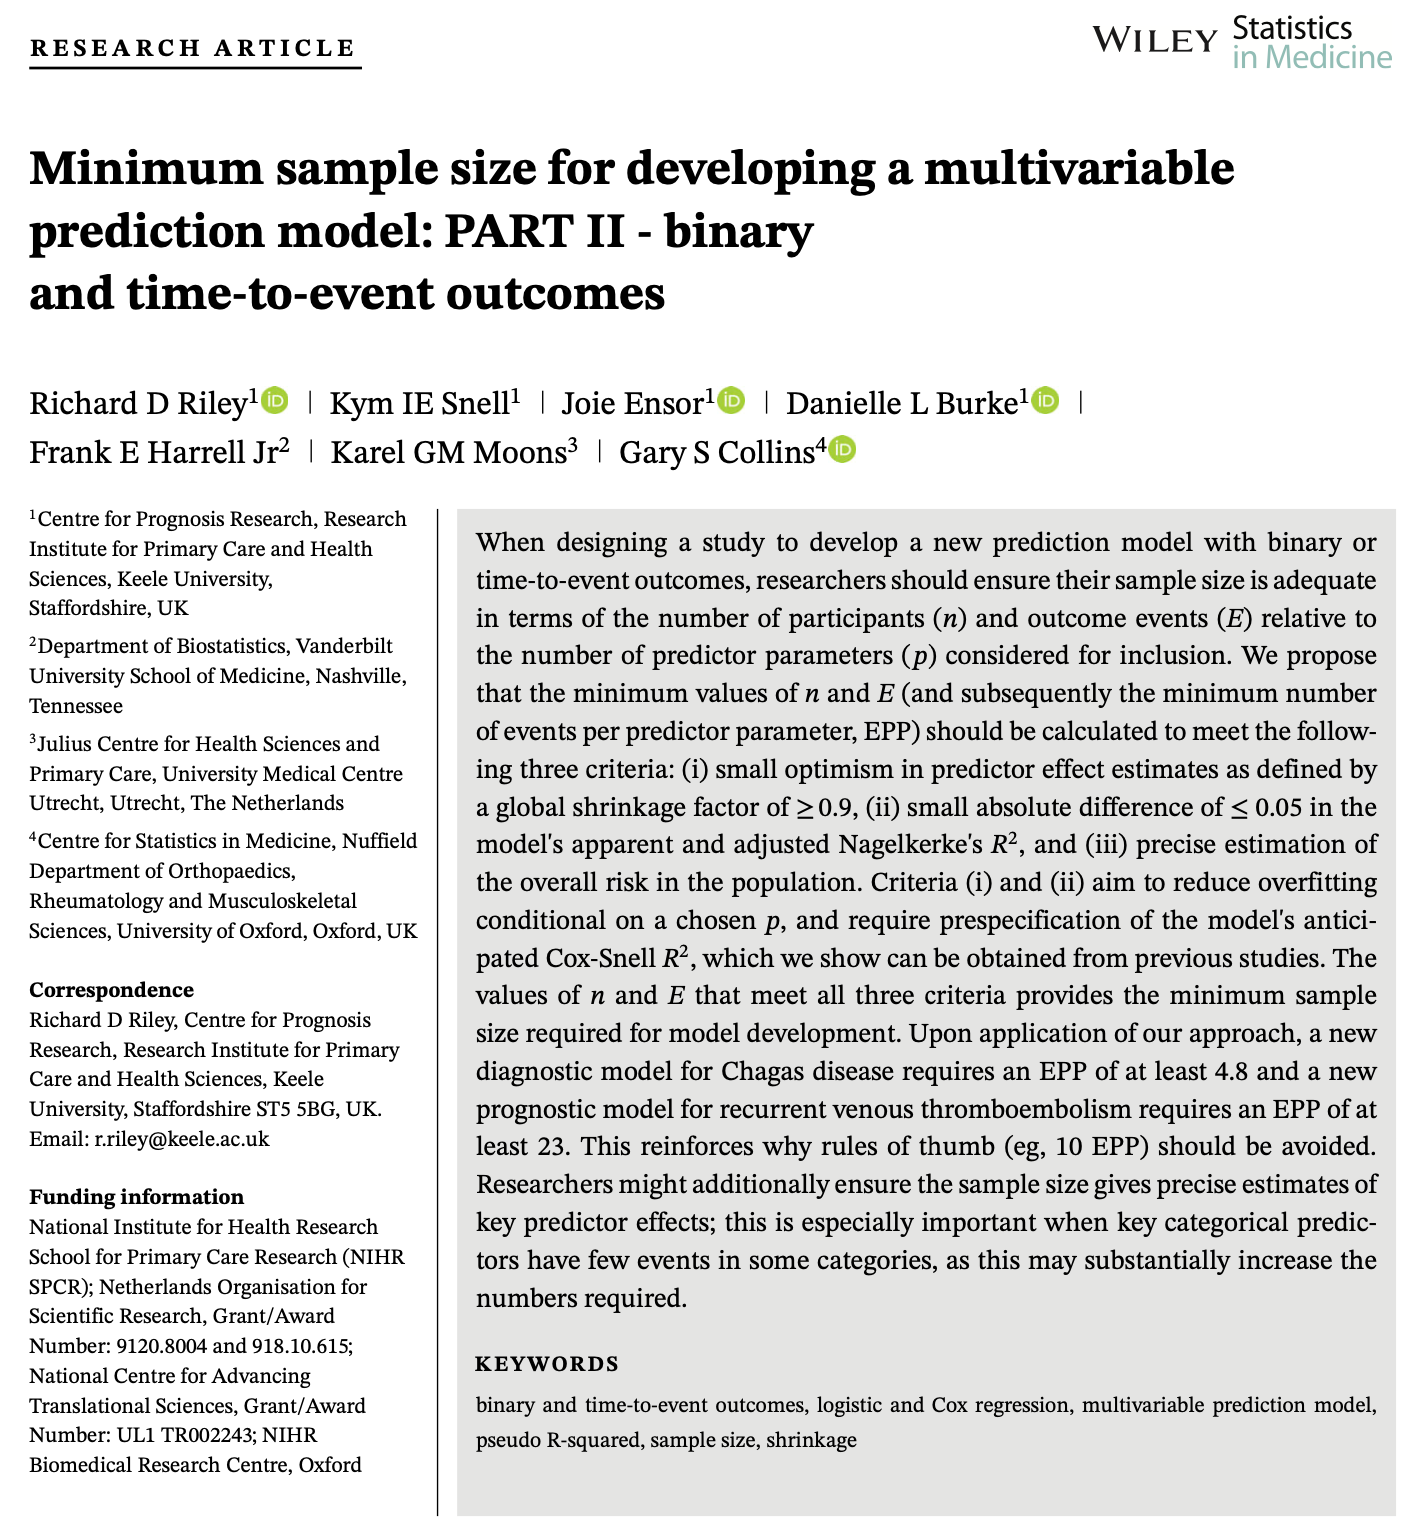
\includegraphics[width=\textwidth]{figures/riley2.png}%
		\end{column}
		\begin{column}[T]{0.4\textwidth}
			\centering
			\vspace{-4em}
			In 2018, Riley et al.\ released pmsampsize\autocite{riley2021} for R and Stata.
		\end{column}
	\end{columns}

\end{frame}

\begin{frame}[t]{We \img{figures/heart.png} pmsampsize, but\ldots}
	\large
	\vspace{1em}
	We increasingly need to estimate minimum samples for:\ \sgap
	\begin{itemize}
		\colitem{KCLpurple}{Other models (e.g., machine learning algorithms, random
			forests, gradient boosting)}
		\colitem{KCLseablue}{Other data types (e.g., longitudinal, clustered)}
	\end{itemize}

	\onslide<2->
	\vspace{1.5em}
	We're developing a simulation-based framework to estimate sample
	sizes for prediction.

	\begin{cbox}[colframe=KCLhotpink!50!black]{KCLhotpink}{}
		\RaggedRight
		{\Large \textbf{The pmsims package for R}}

        \bgap

		\begin{tabular}{rp{0.8\textwidth}}
			\textbf{Flexible}      & Any model or data type             \\
			\textbf{User-friendly} & Defaults for common scenarios      \\
			\textbf{Efficient}      & Estimation via surrogate modelling
		\end{tabular}
	\end{cbox}

\end{frame}

\begin{frame}[t]{Our approach}
    \vspace{1em}
    \Wider[1.5em]{
    \begin{cbox}[bottom=4mm]{KCLpeagreen}{Setting}
		\begin{enumerate}
			\setlength{\itemsep}{7pt}
            \item A \textbf{study population} represented by outcome-related individual
			      characteristics (i.e., candidate predictors).
              \item A chosen statistical or machine learning \textbf{model}.
              \item Expected achievable \textbf{large-sample performance}, $P^{*}$, given population and model.
              \item Minimum \textbf{acceptable test performance} of the model, $P^{OK}$.
		\end{enumerate}
	\end{cbox}
}

	\onslide<2->
    \vspace{1.2em}
	\centering
	
\includegraphics[height=3.6em]{figures/target.pdf}
	\hspace{0.7em}
	\large
	\parbox[b]{0.8\textwidth}{ \raggedright \tc{KCLpantone}{ Find the
	    minimum sample that ensures test performance of $P^{OK}$ with
	    probability of 80\%, given the population, predictors, and $P^{*}$. }
	    }

	% i.e., drawing a random sample of size $n$ will result in a model with
	% performance $>P^{OK}$ in more than 80\% of cases.

\end{frame}

\begin{frame}{How does it work?}

	\begin{columns}[T]
		\begin{column}{0.4\textwidth}
			\centering
			\includegraphics<+>[width=0.85\textwidth]{figures/workflow-a.pdf}%
			\includegraphics<+>[width=0.85\textwidth]{figures/workflow-b.pdf}%
			\includegraphics<+>[width=0.85\textwidth]{figures/workflow-c.pdf}%
			\includegraphics<+>[width=0.85\textwidth]{figures/workflow-d.pdf}%
		\end{column}
		\begin{column}{0.7\textwidth}
            \large
			\only<1>{
				\vspace{1em}
				The user specifies:
				\begin{enumerate}
					\item The candidate predictors (number, type)
					\item The chosen statistical model
					\item The expected large sample performance ($P^{*}$)
					\item The minimum acceptable performance ($P^{OK}$)
				\end{enumerate}
			}%
			\only<2>{
				\vspace{5.5em}
				Based on their input, we set:
				\begin{enumerate}
					\item A data-generating function
					\item A model function
					\item A metric function
				\end{enumerate}
			}%
			\only<3>{
				\vspace{10em}
				We tune the data generating model, so the large sample
				performance is $P^{*}$.
			}
		\end{column}
	\end{columns}

\end{frame}

\begin{frame}[t]{Performing the search}
	\tikz[overlay, remember picture]
	\node[%
		anchor=north east,
		yshift=0.2cm,
		xshift=-0.5cm]at (current page.north east) {
		\includegraphics[width=0.28\textwidth]{figures/tortoise.png}%
	};

	\vspace{-0.5em}
	An exhaustive grid search would be too slow.
	\Wider{%
		\vspace{2em}
		\begin{cbox}{KCLpurple}{Surrogate modelling with mlpwr}
			% Surrogate modeling aims to approximate a relationship that is costly to
			% investigate with a cheaper function.

			\begin{itemize}
				\item Approximates the relationship between sample size and
				      $P^{OK}$ using Gaussian process regression.
				\item Also referred to as `learning curve
				      fitting'\autocite{figueroa2012, dayimu2023}.
				\item Uses the mlpwr R package by Zimmer and
				      Debelak\autocite{Zimmer.inpress}.
			\end{itemize}
		\end{cbox}

		\vspace{0.3em}
		\centering
		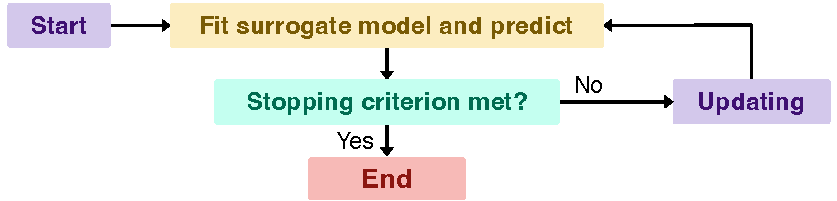
\includegraphics[width=\textwidth]{figures/surrogate_algorithm.pdf}%
	}
\end{frame}

\begin{frame}[c]{}
	\Wider[2em]{
		\includegraphics<+>[width=\textwidth]{figures/surrogate-1.pdf}%
		\includegraphics<+>[width=\textwidth]{figures/surrogate-3.pdf}%
		\includegraphics<+>[width=\textwidth]{figures/surrogate-4.pdf}%
		\includegraphics<+>[width=\textwidth]{figures/surrogate-5.pdf}%
		\includegraphics<+>[width=\textwidth]{figures/surrogate-6.pdf}%
	}

\end{frame}

\begin{frame}[t]{What is the performance of a prediction model?}
	\Wider{
		\vspace{0.6em}

		{\centering
			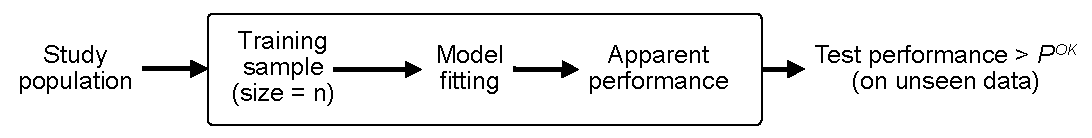
\includegraphics[width=\textwidth]{figures/performance_flow.pdf}%
		}%

		\vspace{0.5em}%

    {\large \tc{KCLpantone}{\textbf{Apparent vs. test performance} (or ``actual'' performance)}}

		\begin{itemize}
			\item Train/test performances are random variables of the drawn
			      sample.
			\item Test performance is expected to be worse than apparent; but
			      difference reduced with higher n.
			\item A prediction model is as good as its test performance.
		\end{itemize}

		\vspace{1em}
		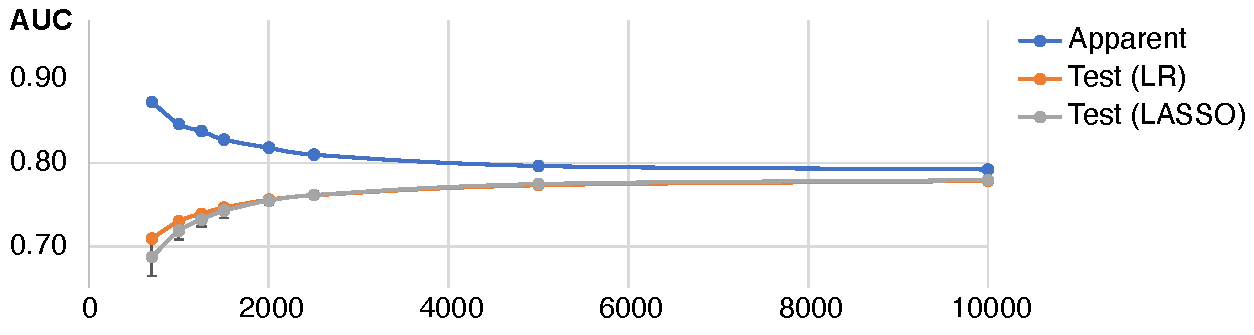
\includegraphics[width=\textwidth]{figures/diana-auc.pdf}%
	}
\end{frame}

\begin{frame}[t]{How do we assess performance?}

	We identify the minimum sample that meets \underline{three} criteria:

	\begin{cbox}{KCLpeagreen}{1.\ Overall fit} 
		Within 0.1 of the achievable large sample fit (e.g., $R^2$, Brier).
	\end{cbox}

	\begin{cbox}{KCLseablue}{2.\ Discrimination} 
		Within 0.1 of the achievable large sample discrimination (e.g., C-statistic, AUC).
	\end{cbox}

	\begin{cbox}{KCLhotpink}{3.\ Calibration slope}
		A calibration slope of 0.9 to 1.1.
	\end{cbox}

	The choice of metrics and thresholds are user-configurable.

\end{frame}


\begin{frame}[c]{Two approaches to estimating minimum samples}
	\vspace{0.7em}
	\small
	\Wider[5em]{
		\renewcommand{\arraystretch}{1.4}
		\begin{tabular}{%
			r%
			@{~~}R{0.39\textwidth}%
			R{0.41\textwidth}@{}}

			                                                                & {\Large \tc{KCLpurple}{pmsims}}                                                                                                            & {\Large \tc{KCLhotpink}{pmsampsize}} \\[2mm]
			\gr{Approach}                                                   & \tc{KCLpurple}{Simulate absolute test performance}                                                                                         &
			\tc{KCLhotpink}{Analytical closenesss of train-test; prevent overfitting}                                                                                                                                                                           \\[2mm]
			\gr{Target}                                                     &
			Sample ensuring test performance $P^{OK}$ with 80\% probability. &
			Sample ensuring apparent and test performances are sufficiently close.                                                                                                                                                                               \\[7mm]
			\gr{How}                                                        & Tune data generator, use mlpwr to search for minimum sample meeting criteria.                                                              &
			Targets small train-test difference in $R^2$;
			or uniform shrinkage above given threshold (e.g., 0.9).                                                                                                                                                                                             \\
			\gr{Calibration}                                                & \begin{minipage}[t]{0.39\textwidth}\RaggedRight Calibration slope criterion is similar to uniform shrinkage criterion. \\ \vspace{.7em}
				                                                                  Slope is defined as minimizing the error between $y^{test}$ and $\alpha + slope \times \hat{y}^{test}$.
			                                                                  \end{minipage} &
			\begin{minipage}[t]{0.39\textwidth}\RaggedRight
				Uniform shrinkage:\ GLM models where estimates depend on a linear predictor, $x^{T}\hat{\beta}$, with $\hat{\beta}-OLS$ estimates from the training sample.                                                                                        \\ \vspace{.7em}
				$s \cdot x^{T} \hat{\beta}$ may $\downarrow$overfitting and $\uparrow$performnce on unseen cases.
			\end{minipage}
		\end{tabular}
	}

\end{frame}

\begin{frame}[c]{What are the distinctive features of these approaches?}
	\Wider[3em]{
		\renewcommand{\arraystretch}{1.8}
		\begin{tabular}{@{}R{0.35\textwidth}R{0.3\textwidth}R{0.3\textwidth}@{}}
			                                                     & {\Large \tc{KCLpurple}{pmsims}}  & {\Large \tc{KCLhotpink}{pmsampsize}} \\[2mm]
			\tc{KCLpantone}{Flexibility}                        & Any model/data                          & Closed form only for some models            \\
			\tc{KCLpantone}{Complex designs}                    & Specified by user               & Not possible                                \\
			\tc{KCLpantone}{Speed}                              & Slower*                                 & Fast                                        \\
			\tc{KCLpantone}{Of 100 training samples of size n*} & Test performance above $P^{OK}$ in 80\% & Mean test performance = $P^{OK}$            \\
			\tc{KCLpantone}{Large test performance variability} & Adjusted for (using 0.2 quantile)       & Not adjusted for
		\end{tabular}
	}
\end{frame}


		% \begin{tabular}{@{}p{0.5\textwidth}@{}p{0.5\textwidth}}
		% 	{\Large pmsims}                     & {\Large pmsampsize} \\
		% 	\begin{minipage}[t]{0.45\textwidth}
		% 		\begin{itemize}
		% 			\item Targets absolute performance
		% 			\item Flexible
		% 			      % Machine learning, multilevel models, etc.
		% 			      % heteroscedasticity and multicollinearity in the data
		% 			\item Does not aim to prevent overfitting per se
		% 			\item Targets test performance*
		% 			\item Adjusts recommendations for test performance
		% 			      variance**
		% 		\end{itemize}
		% 		However:\
		% 		\begin{itemize}
		% 			\item Computationally demanding
		% 			\item User must specify data/model for complex designs
		% 			\item Simulation variability
		% 		\end{itemize}
		% 	\end{minipage} &
		% 	\begin{minipage}[t]{0.45\textwidth}
		% 		\begin{itemize}
		% 			\item Fast, closed-form solutions
		% 			\item Ensures sufficient training sample to prevent
		% 			      overfitting
		% 		\end{itemize}
		% 		However:\
		% 		\begin{itemize}
		% 			\item Closed-form only for some
		% 			      models\autocite{riley2021}.
		% 			\item Does not adjust predictions to the variance of the
		% 			      test performance\autocite{vanhouwelingen1990a}.
		% 			\item As only one training sample will be available to the
		% 			      model developers, actual performance once deployed
		% 			      may be much lower**.
		% 		\end{itemize}
		% 	\end{minipage}
		% \end{tabular}
	% }

\end{frame}

\begin{frame}[t]{}

	\Wider{
		\vspace{0.3em}
		\textbf{Compared to pmsampsize}, our approach may suggest:
		\begin{tcolorbox}[arc=0.2mm, colback=white,boxrule=1pt]
			\tc{KCLpeagreen}{\textbf{Smaller N} for machine learning models:}\
			\begin{itemize}
				\setlength\itemsep{0.2mm}
				\item[--] Tend to overfit but may still achieve sufficient test performance
			\end{itemize}
			\tc{KCLred}{\textbf{Larger N} for noisy data and models with high variance:}\
			\begin{itemize}
				\setlength\itemsep{0mm}
				\item[--] 0.2 quantile test performance < mean performance.
			\end{itemize}
		\end{tcolorbox}
		\centering
		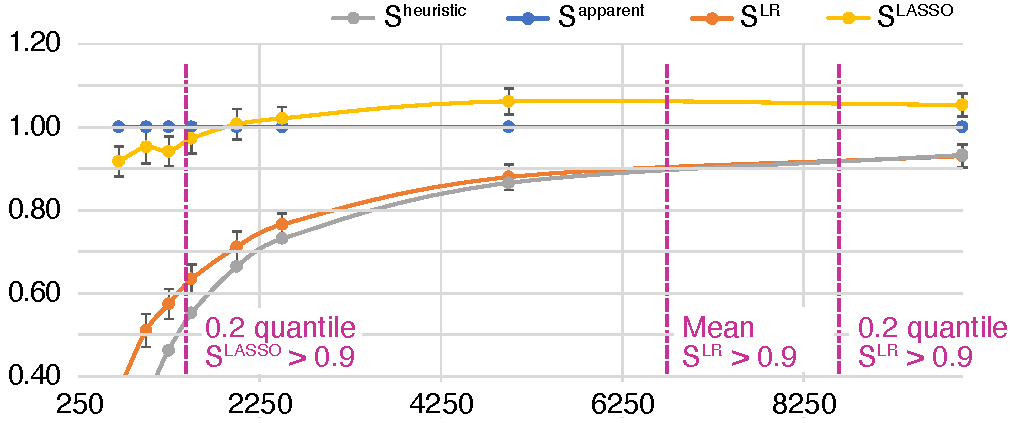
\includegraphics[width=\textwidth]{figures/diana-slope.pdf}%
	}

\end{frame}

\begin{frame}[c,fragile]{The user interface}

	\vspace{1em}
	\centering
	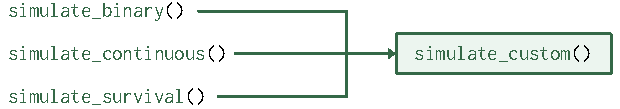
\includegraphics[width=0.9\textwidth]{figures/interfaces.pdf}%
	\vspace{-1.5em}

	\begin{columns}
		\begin{column}[t]{0.55\textwidth}
			\begin{cbox}{gray}{}
				\begin{minted}[autogobble,fontsize=\small]{r}
simulate_continuous <- 
  function(
    signal_parameters = 30,
    noise_parameters = 0,
    min_sample_size = 300,
    max_sample_size = 10000,
    large_discrimination = 0.7,
    minimum_threshold = 0.1,
    model = "lm",
    metric = "r2",
    ...
  ) 
            \end{minted}
			\end{cbox}
		\end{column}
		\begin{column}[t]{0.55\textwidth}
			\begin{cbox}{gray}{}
				\begin{minted}[autogobble,fontsize=\small]{r}
simulate_binary <- 
  function(
    signal_parameters = 30,
    noise_parameters = 0,
    baseline_prob = 0.1,
    min_sample_size = 300,
    max_sample_size = 10000,
    large_discrimination = 0.8,
    minimum_threshold = 0.1,
    metric = "auc",
    model = "glm",
    ...
  )
            \end{minted}
			\end{cbox}
		\end{column}
	\end{columns}

\end{frame}

\begin{frame}[b,fragile]{Example:\ Binary outcome, logistic regression}
	\Wider{
		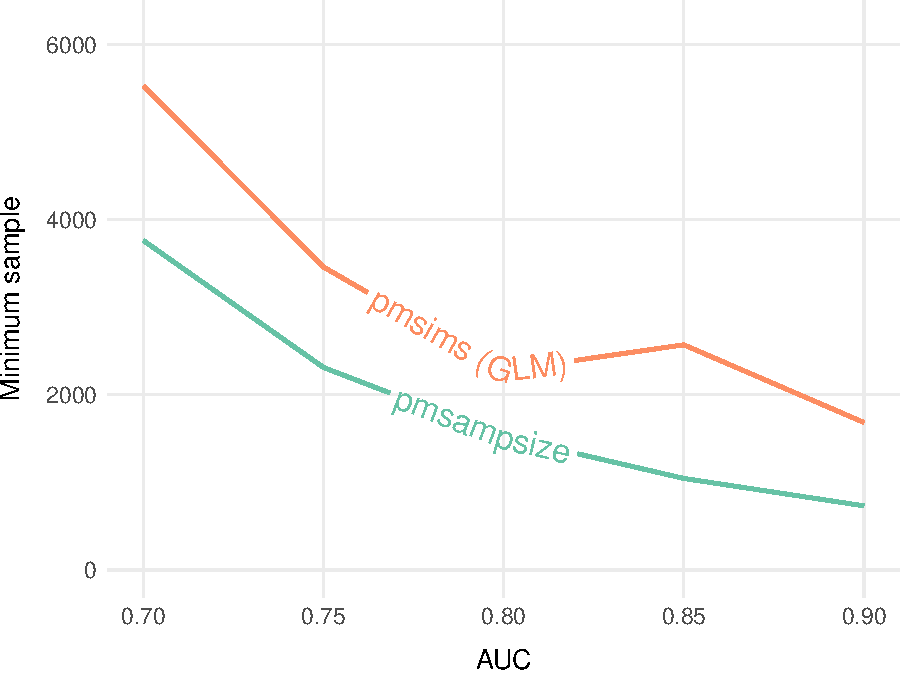
\includegraphics[width=0.9\textwidth]{figures/demo1.pdf}%
	}

	\tikz[overlay, remember picture]
	\node[anchor=north east, yshift=-0.9cm, xshift=-0.1cm] at (current page.north east) {
		\begin{cbox}[width=4.8cm,bottom=1mm]{gray}{}%
			\begin{minted}[autogobble,fontsize=\footnotesize]{r}
simulate_binary(
  signal_parameters = 20,
  baseline_prob = 0.1,
  min_sample_size = 500,
  max_sample_size = 15000,
  large_discrimination = ...,
  minimum_threshold = 0.1,
  metric = "auc",
  model = "glm",
)
            \end{minted}
		\end{cbox}
	};

\end{frame}

% \begin{frame}[b,fragile]{Example 2:\ Binary outcome, LASSO regression}

% 	\Wider{
% 		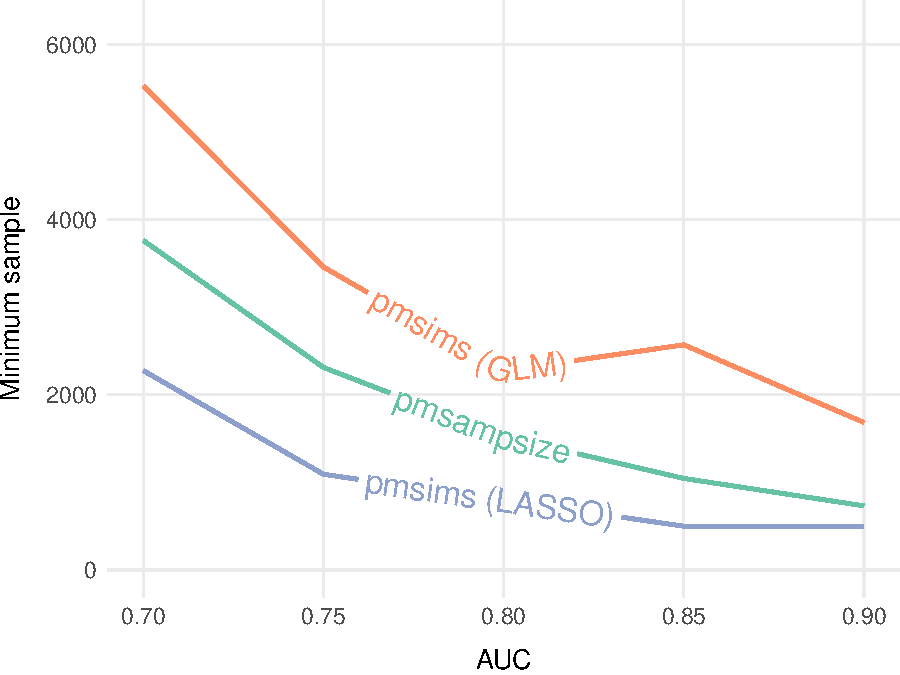
\includegraphics[width=0.9\textwidth]{figures/demo2.pdf}%
% 	}

% 	\tikz[overlay, remember picture]
% 	\node[anchor=north east, yshift=-0.9cm] at (current page.north east) {
% 		\begin{cbox}[width=4.8cm]{gray}{}%
% 			\begin{minted}[%
%                 highlightlines=9,
%                 autogobble,
%                 fontsize=\scriptsize]{r}
% simulate_binary(
%   signal_parameters = 20,
%   baseline_prob = 0.1,
%   min_sample_size = 500,
%   max_sample_size = 15000,
%   large_discrimination = ...,
%   minimum_threshold = 0.1,
%   metric = "auc",
%   model = "lasso",
% )
%             \end{minted}
% 		\end{cbox}
% 	};

% \end{frame}

\begin{frame}[c,fragile]{Example:\ Custom model function}

	What if a model hasn't been implemented? e.g., XGBoost \vspace{-0.5em}%

	\begin{columns}
		\begin{column}[T]{0.5\textwidth}
			\begin{cbox}{gray}{}%
				\begin{minted}[autogobble,fontsize=\scriptsize]{r}
model_function <- function(d) {
  dmat <- xgboost::xgb.DMatrix(
    as.matrix(d[, -1]),
    label = d[, 1]
  )
  param <- list(
    objective = "binary:logistic",
    booster = "gblinear",
    alpha = 0.0001,
    lambda = 1
  )
  xgboost::xgb.train(
    param,
    dmat,
    nrounds = 2
  )
}
            \end{minted}
			\end{cbox}

		\end{column}
		\begin{column}[T]{0.55\textwidth}
			\begin{cbox}{gray}{}%
				\begin{minted}[%
                autogobble,
                fontsize=\scriptsize]{r}
metric_function <- function(data,
                            fit,
                            model) {
  dmat <- xgboost::xgb.DMatrix(
    as.matrix(data[, -1]), 
    label = data[, 1]
  )
  y_hat <- predict(fit, dmat)
  pROC::auc(data[, 1], y_hat)[1]
}
            \end{minted}
			\end{cbox}

			\begin{cbox}{gray}{}%
				\begin{minted}[%
                highlightlines=2-4,
                autogobble,
                fontsize=\scriptsize]{r}
simulate_custom(
  data_function = data_function,
  model_function = model_function,
  metric_function = metric_function,
  ...
)
            \end{minted}
			\end{cbox}
		\end{column}
	\end{columns}

\end{frame}

\section{Conclusion}

\begin{frame}[c]{Development status}

	% We're still developing the package.
	% It works, but more testing needed.

		\begin{columns}
			\begin{column}[T]{0.24\textwidth}
				\begin{itemize}
					\item[$\checkmark$]  Framework
					\item[] {\scriptsize R package}
				\end{itemize}
			\end{column}
			\begin{column}[T]{0.32\textwidth}
				\begin{itemize}
					\item[$\checkmark$]  Data generators
					\item[] {\scriptsize Linear, binary, survival}
				\end{itemize}
			\end{column}
			\begin{column}[T]{0.39\textwidth}
				\begin{itemize}
					\item[$\checkmark$] Model generators
					\item[] {\scriptsize Linear, logistic, Cox, LASSO}
				\end{itemize}
			\end{column}
		\end{columns}


	\vspace{2em}
	{\large \tc{KCLseablue}{What's next?}}
	\sgap

	\begin{cbox}{KCLtealblue}{1.\ Machine learning}
		Defaults for common algorithms (e.g., random forest).

	\end{cbox}

	\begin{cbox}{KCLseablue}{2.\ Longitudinal and clustered data}
		Data generators and models (e.g., landmarking, joint).
	\end{cbox}

\end{frame}

\begin{frame}[t]{}

	\begin{cbox}{KCLpeagreen}{3.\ More sophisticated data generators}
		Synthesise common data types (e.g., genetic); user control.
	\end{cbox}

	\begin{cbox}{KCLred}{4.\ Performance}
		Parallelisation, caching of common tuning parameters.
	\end{cbox}

	\onslide<2->
	\vspace{1em}
	\begin{cbox}[colframe=KCLhotpink!50!white]{KCLhotpink!30!white}{}
		\begin{tabular}{cp{0.8\textwidth}}
			
\includegraphics[width=2em,valign=c]{figures/mastodon.pdf} &
			Follow \tc{KCLhotpink}{fediscience.org/@ewan} for updates                                                                            \\[1.1em]
			
\includegraphics[width=2em,valign=c]{figures/bell.pdf}     &
			Enter email at
			\href{https://tinyurl.com/is-pmsims-ready-yet}{\tc{KCLhotpink}{tinyurl.com/is-pmsims-ready-yet}} to receive one email when its ready \\[1.1em]
			
\includegraphics[width=2em,valign=c]{figures/hi.pdf}       &
			Come and talk to us
		\end{tabular}
	\end{cbox}

\end{frame}

\begin{frame}[t]
	\centering
    \vspace{0.15\textheight}
    {\Large Thank you for listening.}\\[3em]
	\begin{tabular}{cl}
		
\includegraphics[width=1.5em,valign=c]{figures/slides.pdf}   & \tc{KCLhotpink}{\href{https://github.com/ewancarr/pmsims-iscb}{github.com/ewancarr/pmsims-iscb}} \\[1.3em]
		
\includegraphics[width=1.5em,valign=c]{figures/email.pdf}    & \tc{KCLhotpink}{ewan.carr@kcl.ac.uk}                                                             \\[.3em]
		                                                             & \tc{KCLhotpink}{diana.shamsutdinova@kcl.ac.uk}                                                   \\[1.3em]
		
\includegraphics[width=1.5em,valign=c]{figures/mastodon.pdf} & \href{https://fediscience.org/@ewan}{\tc{KCLhotpink}{fediscience.org/@ewan}}
	\end{tabular}

    \vspace{4em}
    
\includegraphics[width=1.5cm]{figures/kcl.png}
\end{frame}

\appendix

\begin{frame}[allowframebreaks]{References}
	\renewcommand*{\bibfont}{\footnotesize}
	\printbibliography
\end{frame}

\end{document}
